Before a system administrator (and others within their organisation) can use Miraihilate, it will first have to be setup. The setup utility will use a command-line interface (CLI) and is written in Python. It will ensure that an initial user of an admin role is created, so that there is a user available upon the application being run for the first time.

\vspace{0.5cm}

\begin{figure}[h]
	\centering
	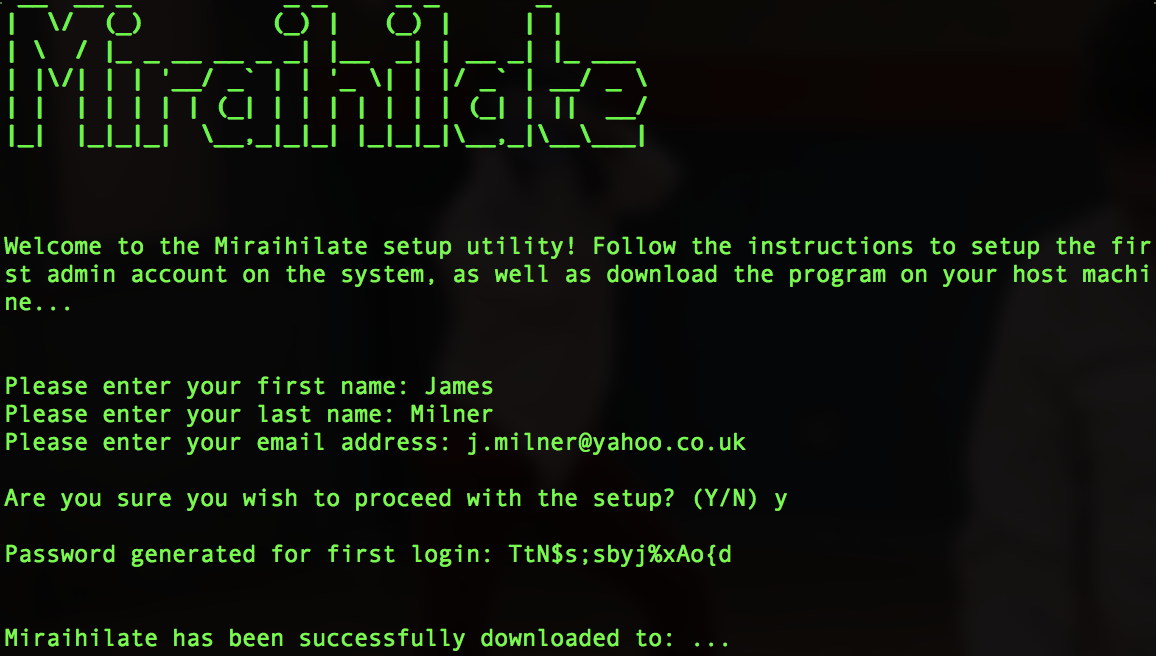
\includegraphics[width=1\linewidth]{img/setup_interface_screenshot.png}
	\caption{Setup Program CLI}
\end{figure}

As shown in Figure 4.1, the setup program asks for the user's first name, last name and email address. The email address will be what they use to login to the system. The setup utility does not ask for a password, but instead generates a cryptographically-secure 16 character long password made up of letters, numbers and symbols.

\vspace{0.5cm}

Before sending the resulting user information to the database, it first generates a Universally Unique Identifier (UUID) and the BCrypt hash for the raw password.

\begin{lstlisting}[language=Python, caption=Hashing a raw password using BCrypt]
pwd_hash = bcrypt.hashpw(raw_pwd.encode('ascii'), bcrypt.gensalt(prefix=b"2a"))
\end{lstlisting}

As seen in the code above, a salt is generated for the hash with the "\textit{2a}" prefix. This is because the JBCrypt library in Java has not been updated to use the newer prefix, and therefore I have to ensure that the hashes can work both with the Python scripts and the front-end client in Java.
